\documentclass{article}
\usepackage[titletoc, title, toc]{appendix}
\usepackage{hyperref}
\usepackage{graphicx}

\begin{document}
\title{System Design Document for NeedForGhetto (SDD)}
\author{}
\date{}
\maketitle

\tableofcontents

\noindent
\\
\\
\textbf{Version}: 1.0 \\
\textbf{Date}: \today \\
\textbf{Authors}: Anton \\
This version overrides all previous versions.

\section{Introduction}
\subsection{Desgin goals}
The design must be modular to provide the possibility of switching the GUI, controller and/or logic. The design must be written in such a way that it is easy to maintain and change parts of the code.
 
\subsection{Definitions, acronyms and abbreviations}
\begin{itemize}
  \item GUI, Graphical User Interface
  \item Java, platform independent programming language.
  \item MVC, a way to partition an application with a GUI into distinct parts avoiding
  mixing GUI-code and application code.
  \item JSON, fileformat used for transmitting data in a structured way.
  \item TrueType, a font format with high degree of control over how to the font is displayed.
  \item Android, mobile operating system. 
  \item libGDX, framework for developing games in Java.
  \item asset, binary file that contains e.g. sound, texture or font data.
  \item preferences, interface used to write persistent data.
\end{itemize}

\section{System Design}
\subsection{Overview}
The application uses a modified version of the MVC pattern for Android.

\subsubsection{Model Functionality}
The entry point to the model is the World class. We split the model into different classes such as Player, Enemy etc, to keep the design modular and prevent the classes from getting unnecessarily long and complex.

\subsubsection{Global lookups}
The state of the game is tracked with a global variable. The game state can take on the values \textit{PAUSED} or \textit{RUNNING}, and is used to decide if we want to render or not in the \textit{gamescreen} class.
 
There is a special state called \textit{godmode} which is mainly used for testing purposes, it disables the collision control and makes the player invincible.
    
\subsubsection{Event handling}
Generally when the application gets an input from the user it is handled by the controller package which then updates the model accordingly. The view is continuously rendered so a callback from the model is not needed.

Event not handled this way is buttons in menus and the back-key, they are handled directly in the corresponding Screen class. The motivation for this design choice is that these input have nothing to do with the model.

\subsection{Software decomposition}
\subsubsection{General}
The application is decomposed into two main packages, android and core, this is required by libGDX, see figure \ref{fig:nfg}. The android package is for android specific code and assets. The application code resides in the core package, the core package is dependant on libGDX as it uses some of its functions and classes.

\begin{figure}[h]
  \centering
  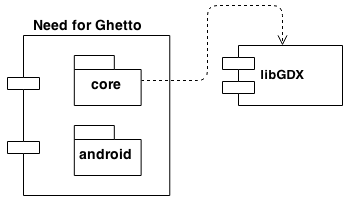
\includegraphics[width=0.8\textwidth]{nfg.png}
  \caption{top level packages and libGDX dependency}
  \label{fig:nfg}
\end{figure}

The core package is further decomposed into: (see figure \ref{fig:core})
\begin{itemize}
  \item view, the GUI part of the game screen, more specific the rendering.
  \item screen, the GUI part of the application.
  \item controller, the controller classes for MVC.
  \item parallax, for parallax background.
  \item highscore, highscore module for reading / writing highscore from file.
  \item gamestate, keeps track of the game state.
  \item model, game logic for the application, model part of MVC.
\end{itemize}

The rendering of the game is decoupled from the GameScreen class to make it easier to debug, modify and add code.

The model is further decomposed of 3 package and 4 classes, the reason for the packages is to reduce clutter and make the package easier to navigate. (see figure \ref{fig:model})

There is also a package for testing.

  \begin{figure}[h]
  \centering
  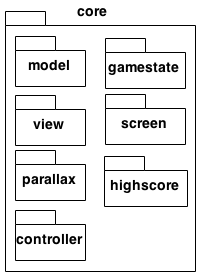
\includegraphics[width=0.5\textwidth]{core.png}
  \caption{Packages with the \textit{core} package}
  \label{fig:core}
  \end{figure}


\subsubsection{Decomposition into subsystem}
The only subsystem present are parallax and highscore.

\subsubsection{Layering}
see figure \ref{fig:stan}

\subsubsection{Dependency analysis}
see figure \ref{fig:stan}


\begin{figure}[h]
  \centering
  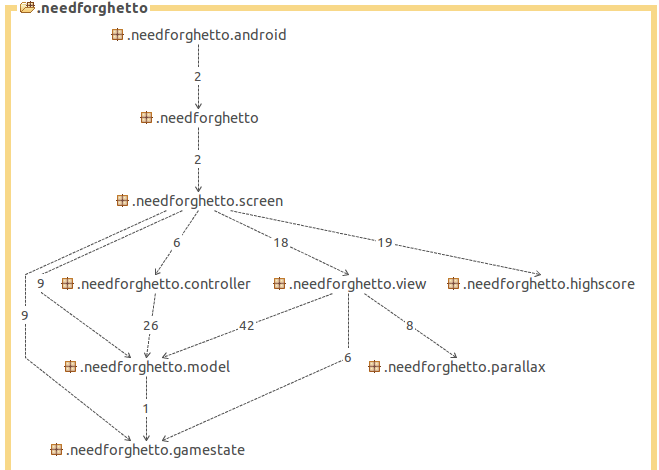
\includegraphics[width=0.8\textwidth]{stan.png}
  \caption{Layering and Dependency analysis}
  \label{fig:stan}
\end{figure}

\subsection{Concurrency issues}
All concurrency is abstracted by libGDX.

\subsection{Persistent data management}
Assets, such as textures, fonts and level information, are persistent and operated on with functions provided by libGDX. The diffrent formats used for storing data are the following: 
\begin{itemize}
  \item Highscore data is handled through the preferences interface.
  \item Level design data is stored as JSON files.
  \item Fonts are stored as TrueType files.
\end{itemize}

\subsection{Access control and security}
NA


\subsection{Boundary conditions}
The application is launched and exited as a normal android application.

\section{References}
\begin{enumerate}
  \item ref1
  \item ref2
  \item ...
\end{enumerate}

\newpage
\begin{appendices}
  \section{Class diagrams}
   
  \begin{figure}[h]
  \centering
  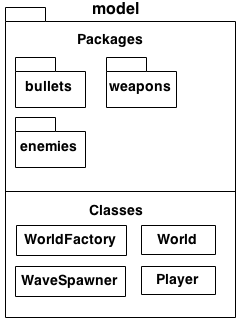
\includegraphics[width=0.5\textwidth]{model.png}
  \caption{Packages and classes within the \textit{model} package}
  \label{fig:model}
  \end{figure}  
  
\end{appendices}

\end{document}